\documentclass{beamer}
\setbeamertemplate{caption}[numbered]
\usepackage{hyperref}  % para autoref
\usepackage{graphicx}
\usepackage[labelfont=bf, labelsep=colon]{caption}

\usetheme{Madrid}  % Podés cambiar "Madrid" por otros temas como Warsaw, Frankfurt, etc.

\title{Proyecto Integrador}
\author{Andyno Cortez}
\date{\today}

\begin{document}

%----- Portada -----
\begin{frame}
  \titlepage
\end{frame}

%----- Índice -----
\begin{frame}{Contenido}
  \tableofcontents
\end{frame}

% ----- Sección 1 -----
\section{Introducción}
\begin{frame}{Introducción}
  \begin{itemize}
    \item Herramientas usadas
    \item Bibliografia
    \item Convencio de signo
    \item Metodo utilizado
  \end{itemize}
  \begin{figure}[h!]
    \centering
    
\includegraphics[width=0.2\textwidth]{logo2.png}
    \caption{}
    \label{fig:logo2}
  \end{figure}
\end{frame}


% ----- Seccón 2 -----

\section{Desarrollo inicial de la resolucion}

\begin{frame}{Matriz de rigidez de una barra}

  Por Figura~\ref{fig:img1}


    \[
        \setlength{\arraycolsep}{6pt}
        \renewcommand{\arraystretch}{1.5}
        \left[
        \begin{array}{c}
        q_{N_{x'}} \\
        q_{N_{y'}} \\
        q_{N_{z'}} \\
        q_{F_{x'}} \\
        q_{F_{y'}} \\
        q_{F_{z'}}
        \end{array}
        \right]
        =
        \left[
        \begin{array}{cccccc}
        \frac{AE}{L} & 0 & 0 & -\frac{AE}{L} & 0 & 0 \\
        0 & \frac{12EI}{L^3} & \frac{6EI}{L^2} & 0 & -\frac{12EI}{L^3} & \frac{6EI}{L^2} \\
        0 & \frac{6EI}{L^2} & \frac{4EI}{L} & 0 & -\frac{6EI}{L^2} & \frac{2EI}{L} \\
        -\frac{AE}{L} & 0 & 0 & \frac{AE}{L} & 0 & 0 \\
        0 & -\frac{12EI}{L^3} & -\frac{6EI}{L^2} & 0 & \frac{12EI}{L^3} & -\frac{6EI}{L^2} \\
        0 & \frac{6EI}{L^2} & \frac{2EI}{L} & 0 & -\frac{6EI}{L^2} & \frac{4EI}{L}
        \end{array}
        \right]
        \left[
        \begin{array}{c}
        d_{N_{x'}} \\
        d_{N_{y'}} \\
        d_{N_{z'}} \\
        d_{F_{x'}} \\
        d_{F_{y'}} \\
        d_{F_{z'}}
        \end{array}
        \right]
        \]
        %  Ecuacion
    \begin{equation*}
        \mathbf{q} = \mathbf{k'} \mathbf{d}
    \end{equation*}

\end{frame}


\begin{frame}{Matriz de desplazamientos globales y locales}


  Por Figura~\ref{fig:img2}

        \[
                \setlength{\arraycolsep}{6pt}
        \renewcommand{\arraystretch}{1.5}
        \left[
        \begin{array}{c}
        d_{N_{x'}} \\
        d_{N_{y'}} \\
        d_{N_{z'}} \\
        d_{F_{x'}} \\
        d_{F_{y'}} \\
        d_{F_{z'}}
        \end{array}
        \right]
        =
        \left[
        \begin{array}{cccccc}
        \lambda_x & \lambda_y & 0 & 0 & 0 & 0 \\
        -\lambda_y & \lambda_x & 0 & 0 & 0 & 0 \\
        0 & 0 & 1 & 0 & 0 & 0 \\
        0 & 0 & 0 & \lambda_x & \lambda_y & 0 \\
        0 & 0 & 0 & -\lambda_y & \lambda_x & 0 \\
        0 & 0 & 0 & 0 & 0 & 1
        \end{array}
        \right]
        \left[
        \begin{array}{c}
        D_{N_{x}} \\
        D_{N_{y}} \\
        D_{N_{z}} \\
        D_{F_{x}} \\
        D_{F_{y}} \\
        D_{F_{z}}
        \end{array}
        \right]
        \]


        %  Ecuacion
        \[
        \mathbf{d} = \mathbf{T} \mathbf{D}
        \]

\end{frame}

\begin{frame}{Cosenos directores}
\begin{align*}
    \lambda_x &= \cos\theta_x = \frac{x_F - x_N}{L} = \frac{x_F - x_N}{\sqrt{(x_F - x_N)^2 + (y_F - y_N)^2}} \\
    \lambda_y &= \cos\theta_y = \frac{y_F - y_N}{L} = \frac{y_F - y_N}{\sqrt{(x_F - x_N)^2 + (y_F - y_N)^2}}
    \end{align*}
\end{frame}

\begin{frame}{Matriz de transformacion de la fuerza}

  Por Figura~\ref{fig:img3}


\[
\setlength{\arraycolsep}{6pt}
\renewcommand{\arraystretch}{1.5}
\left[
\begin{array}{c}
Q_{N_{x}} \\
Q_{N_{y}} \\
Q_{N_{z}} \\
Q_{F_{x}} \\
Q_{F_{y}} \\
Q_{F_{z}}
\end{array}
\right]
=
\left[
\begin{array}{cccccc}
\lambda_x & -\lambda_y & 0 & 0 & 0 & 0 \\
\lambda_y & \lambda_x & 0 & 0 & 0 & 0 \\
0 & 0 & 1 & 0 & 0 & 0 \\
0 & 0 & 0 & \lambda_x & -\lambda_y & 0 \\
0 & 0 & 0 & \lambda_y & \lambda_x & 0 \\
0 & 0 & 0 & 0 & 0 & 1
\end{array}
\right]
\left[
\begin{array}{c}
q_{N_{x'}} \\
q_{N_{y'}} \\
q_{N_{z'}} \\
q_{F_{x'}} \\
q_{F_{y'}} \\
q_{F_{z'}}
\end{array}
\right]
\]

        %  Ecuacion
        \[
        \mathbf{Q} = \mathbf{T}^T \mathbf{q}
        \]

\end{frame}

\begin{frame}{Matriz de rigidez global}

    \begin{gather*}
    \mathbf{q} = \mathbf{k'}\mathbf{T} \mathbf{D} \\
    \mathbf{Q} = \mathbf{T}^T\mathbf{k'}\mathbf{T}\mathbf{D} \\
    \mathbf{Q} =\mathbf{k}\mathbf{D} \\
    \mathbf{k} = \mathbf{T}^T\mathbf{k'}\mathbf{T} \\
    \end{gather*}

    Para obtener los resultados se resuelve
    \[\mathbf{Q} =\mathbf{k}\mathbf{D}\]

    Para los resultados de cada barra luego se calcula
    \[\mathbf{q} = \mathbf{k'}\mathbf{T} \mathbf{D}\]


\end{frame}

\begin{frame}{}
  \begin{figure}[h!]
  \centering
  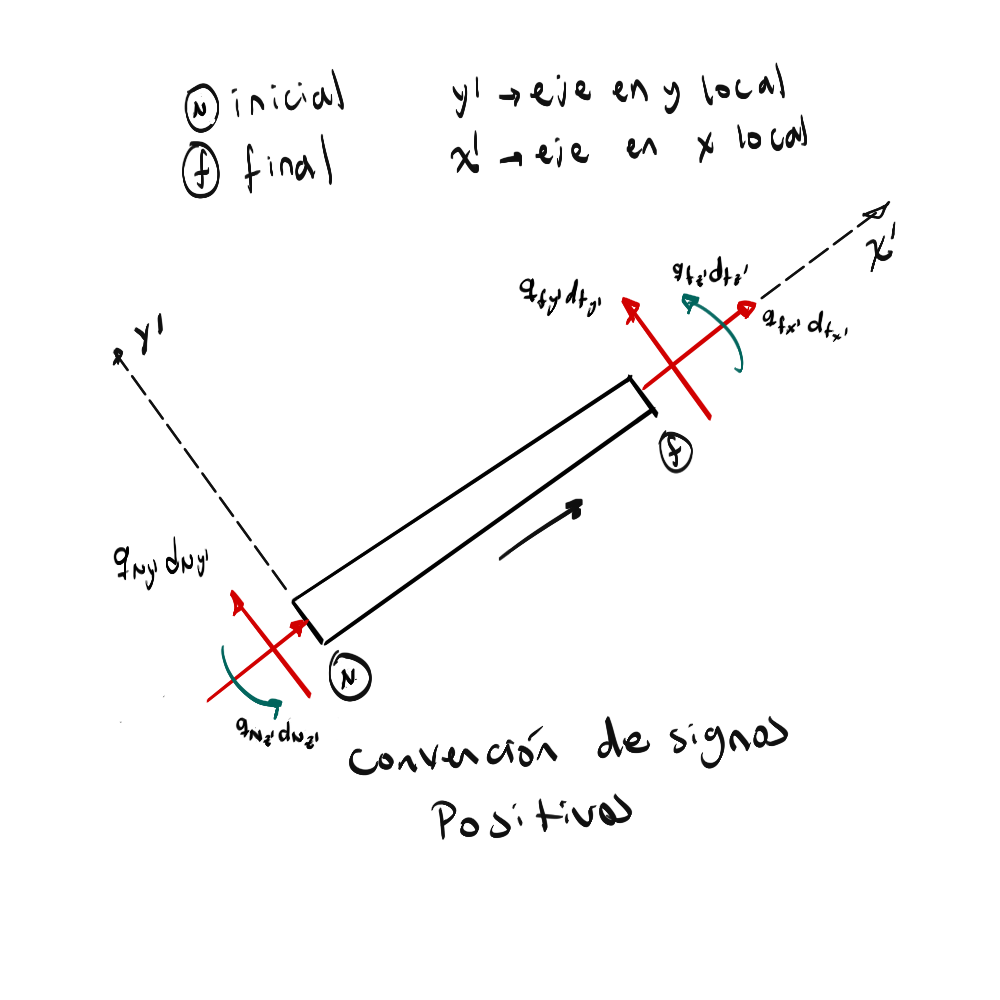
\includegraphics[width=0.6\textwidth]{imagen1.png}
  \caption{}
  \label{fig:img1}
\end{figure}
\end{frame}


\begin{frame}{}
  \begin{figure}[h!]
  \centering
  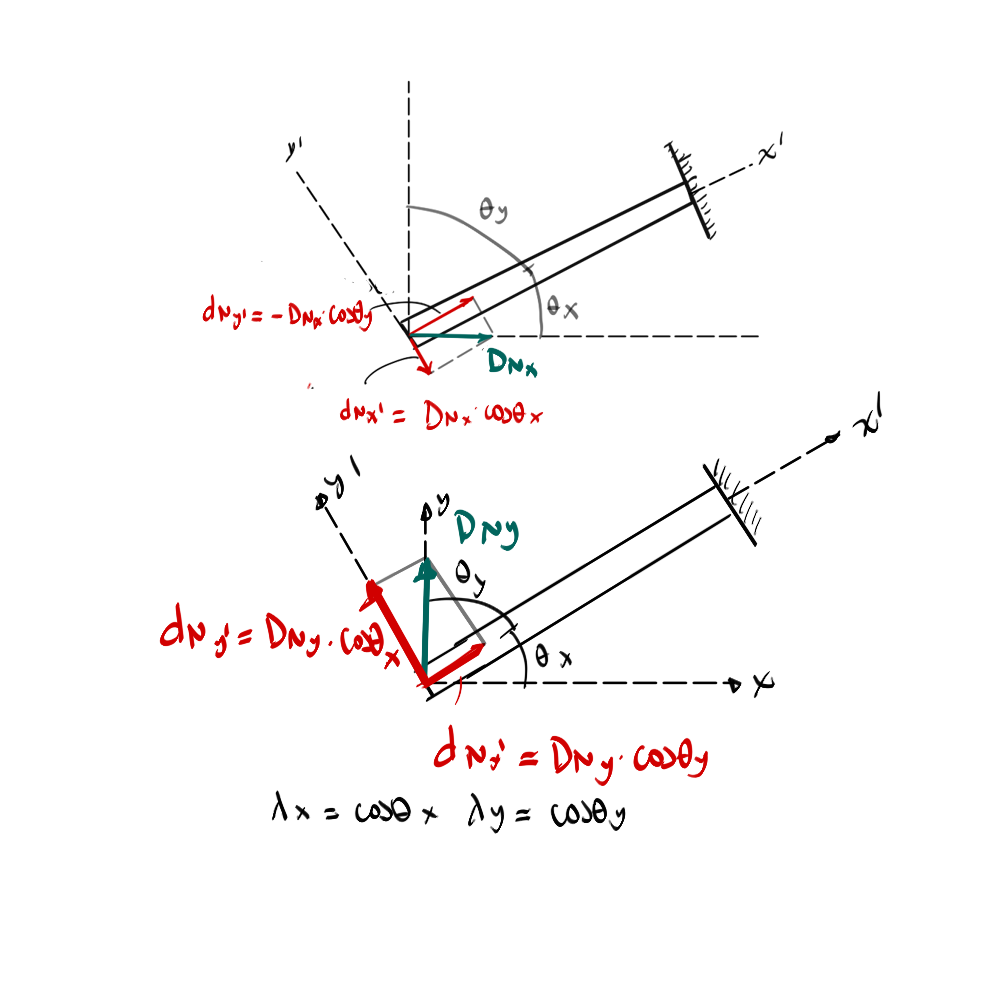
\includegraphics[width=0.6\textwidth]{imagen2.png}
  \caption{}
  \label{fig:img2}
\end{figure}
\end{frame}


\begin{frame}{}
  \begin{figure}[h!]
  \centering
  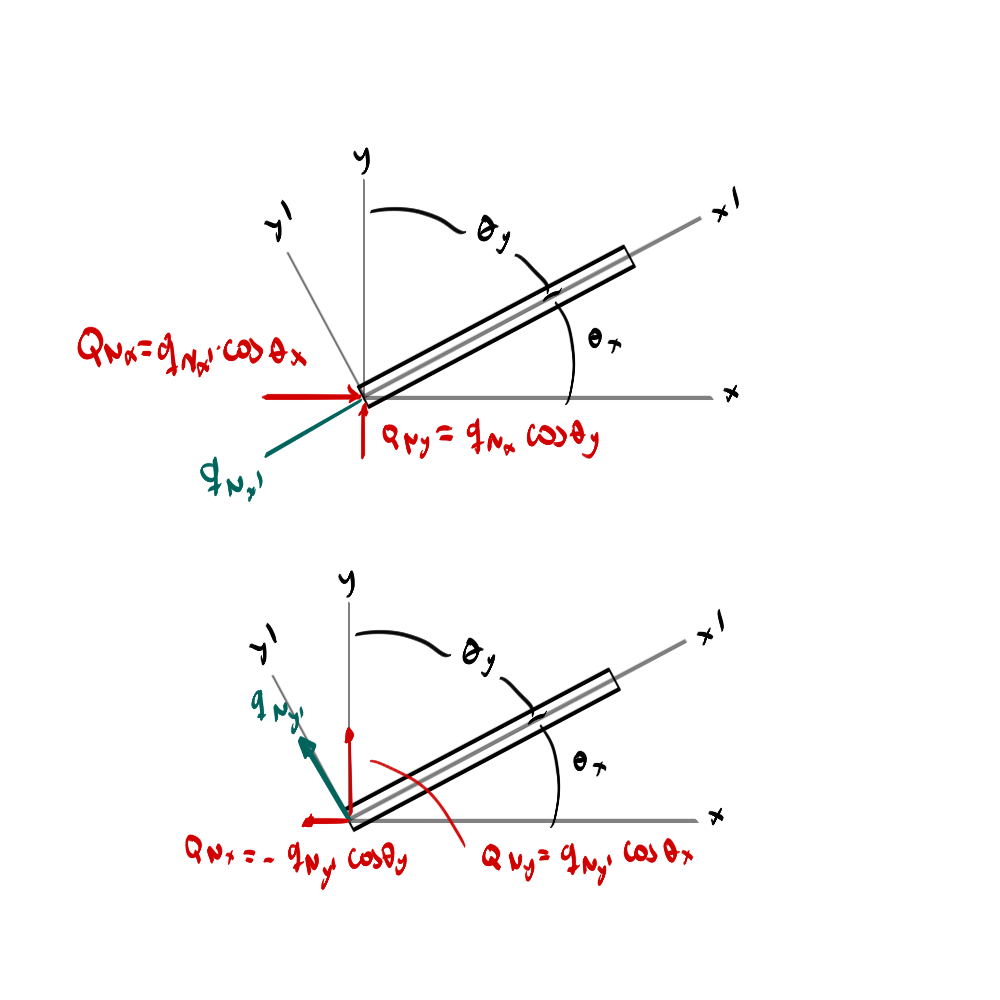
\includegraphics[width=0.6\textwidth]{imagen3.png}
  \caption{}
  \label{fig:img3}
\end{figure}
\end{frame}


\begin{frame}{Calculo de Matriz de transformacion}
  \begin{figure}[h!]
  \centering
  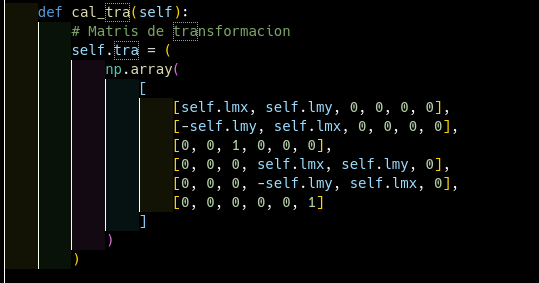
\includegraphics[width=0.6\textwidth]{imagen4.png}
  \caption{}
  \label{fig:img4}
\end{figure}
\end{frame}

\begin{frame}{Calculo de Matriz de rigidez local}
  \begin{figure}[h!]
  \centering
  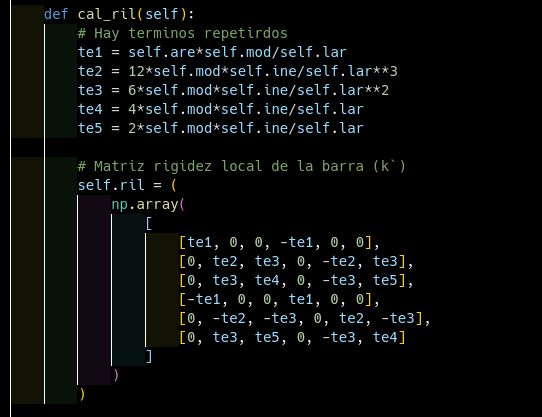
\includegraphics[width=0.6\textwidth]{imagen5.png}
  \caption{}
  \label{fig:img5}
\end{figure}
\end{frame}

\begin{frame}{Calculo de Matriz de rigidez global}
  \begin{figure}[h!]
  \centering
  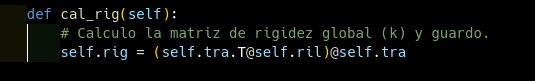
\includegraphics[width=0.6\textwidth]{imagen6.png}
  \caption{}
  \label{fig:img6}
\end{figure}
\end{frame}


\begin{frame}{Resolucion de incognitas}
  \begin{figure}[h!]
    \centering
    
\includegraphics[width=0.2\textwidth]{logo1.png}
    \caption{}
    \label{fig:logo1}
  \end{figure}
  \begin{figure}[h!]
  \centering
  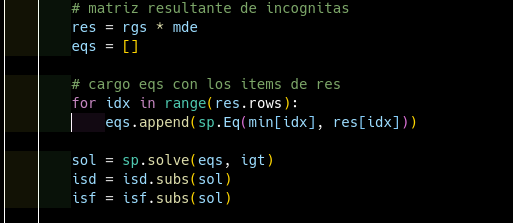
\includegraphics[width=0.6\textwidth]{imagen7.png}
  \caption{}
  \label{fig:img7}
\end{figure}
\end{frame}


\begin{frame}{Resolucion de incognitas}
  \begin{figure}[h!]
  \centering
  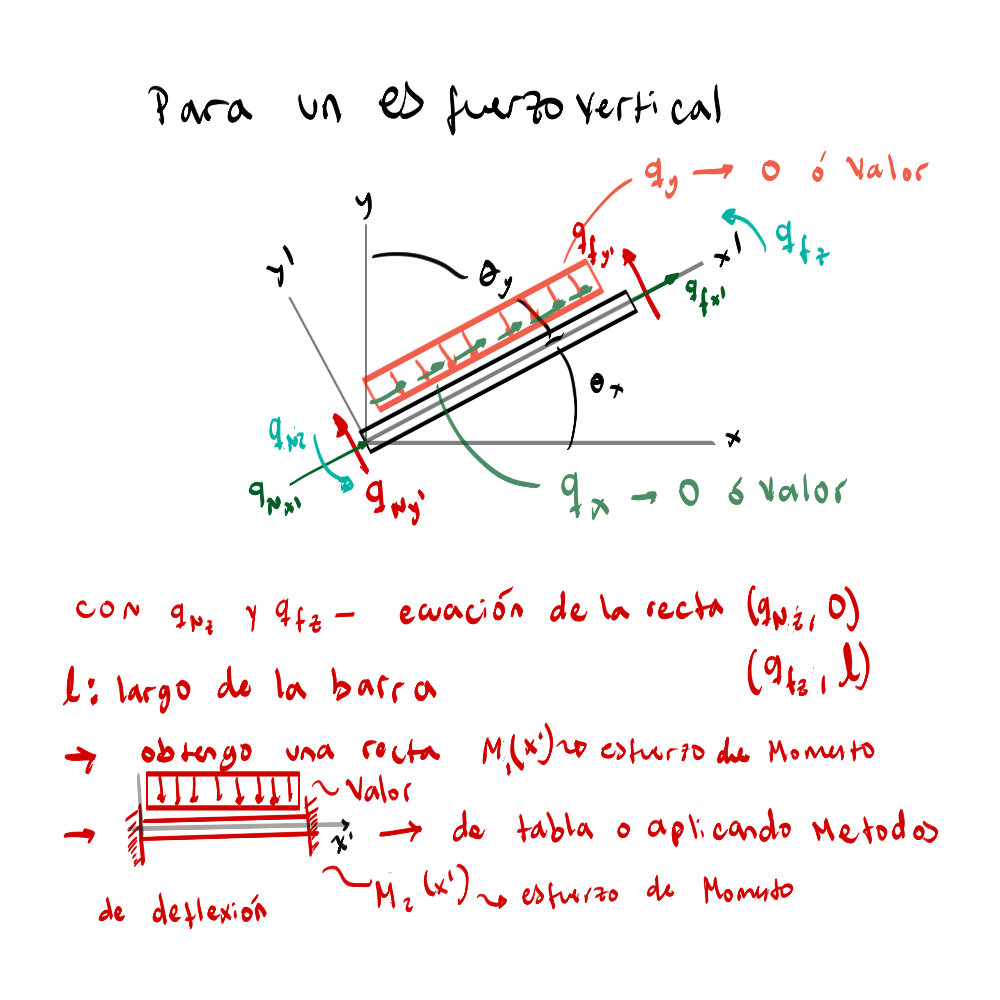
\includegraphics[width=0.6\textwidth]{imagen8.png}
  \caption{}
  \label{fig:img8}
\end{figure}
\end{frame}

\begin{frame}{Resolucion de incognitas}
  \begin{figure}[h!]
  \centering
  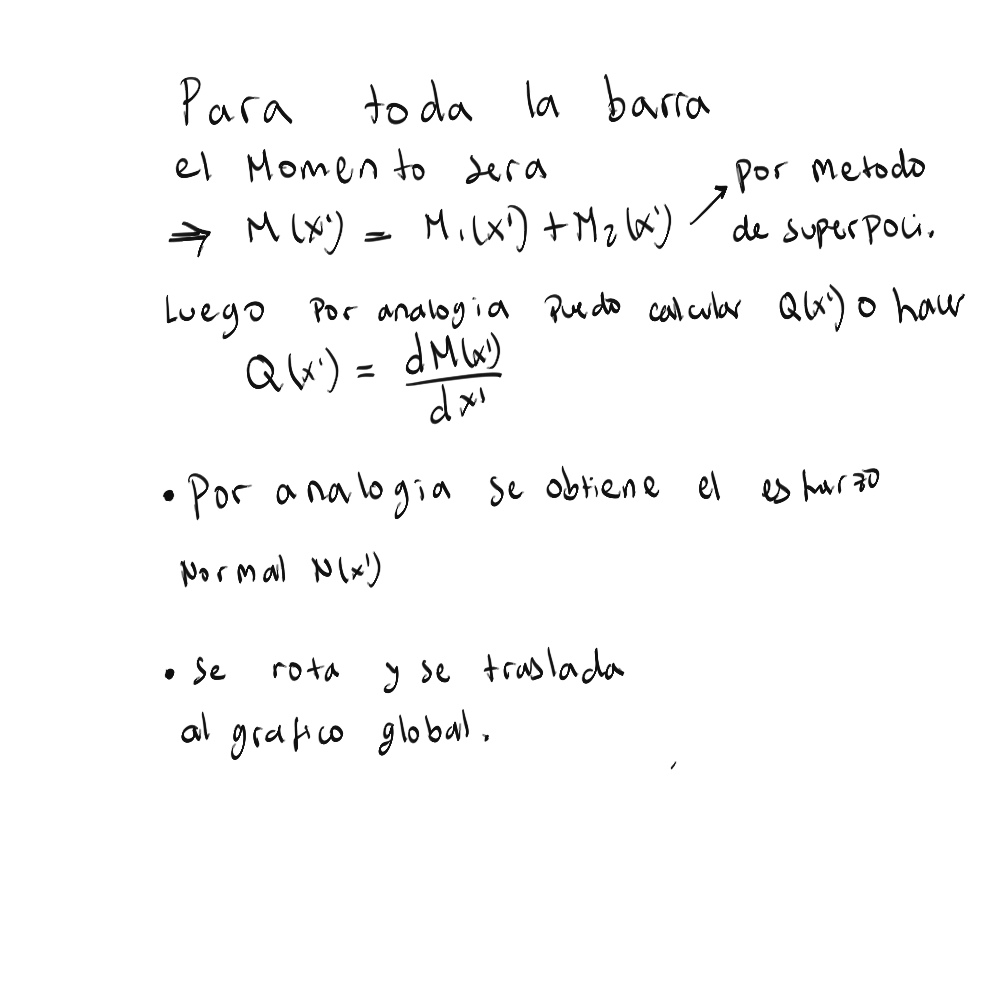
\includegraphics[width=0.6\textwidth]{imagen9.png}
  \caption{}
  \label{fig:img9}
\end{figure}
\end{frame}

\begin{frame}{Comentario}
  Mas de 100h invertidas.
  20 alumnos = 2000h
\end{frame}

%----- Último slide -----
\begin{frame}{Gracias}
  ¡Gracias por tu atención!
\end{frame}

\end{document}
